\section{POI, Query and Path}
\label{sec:method}

\begin{figure*}
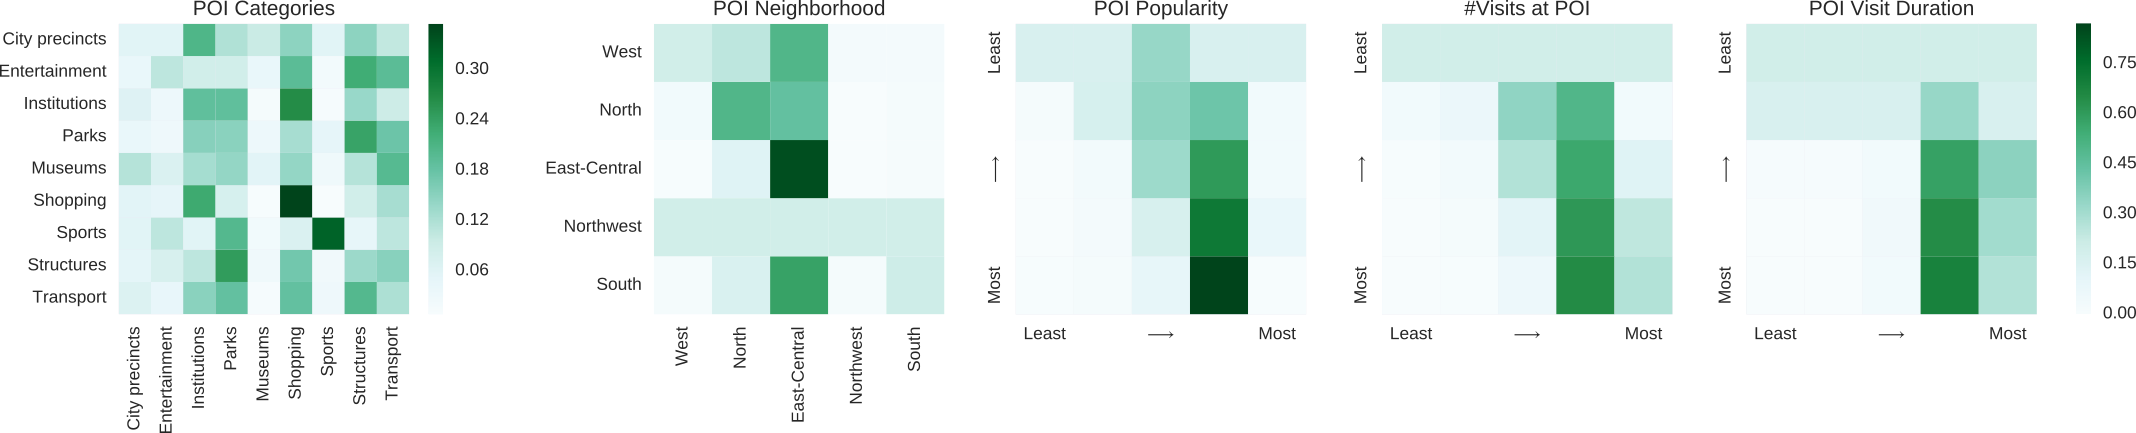
\includegraphics[width=\textwidth]{fig/poi_transmat.png}
\caption{Transition matrices for $5$ individual POI features (Melbourne)}
\label{fig:transmat}
\end{figure*}


We would like to recommend a particular tour such that the user will visit a sequence of points-of-interests (POIs), denoted $p_1, \ldots, p_L$, that maximises utility. We are given the desired start ($p_1=p_s$) and end point ($p_L=p_e$), and an associated number $L$ of POIs desired, from which we propose a trajectory through the city. In Figure~\ref{fig:threesettings}(c), an example tour is shown in blue, which starts at the POI denoted as a grey star, visits two intermediate POIs, and terminates on the fourth POI denoted as a flag. The tour of length 4 can be modelled as a sequence of directed edges in a graph containing POIs in the city as nodes.

The training data consists of a set of tours of varying length in a particular city. We assume that all POIs in the city are visited at least once, and hence can construct a graph with POIs as nodes and potentially multiple directed edges between each pair of nodes. We extract the category, popularity, total number of visits and average visit duration for each POI. The set of categories are shown in figure \ref{fig:poicats} in the appendix, and the popularity is defined as the number of distinct users that visited the POI\cite{ht10}.

As a baseline approach, we recommend the trajectory based on the popularity of POIs only, that is we always suggest the top-$k$ most popular POIs for all visitors given the start and end location. This baseline approach, called \textsc{PoiPopularity}, and its only adaptation to a particular request is to adjust $k$ to match the desired length.

\cheng{I have removed reference to user specific recommendations.}


\subsection{Ranking using the origin and destination}
\label{sec:ranksvm}

\dawei{Features of target POI are already described here.} 

In addition to popularity, we also can rank the candidate POIs based on the other three POI specific features (category, total visits and average duration).
We can learn a ranking of POIs by using rankSVM with linear kernel and $L2$ loss\cite{lranksvm},
\begin{displaymath}
\min_{\mathbf{w_r}} \frac{1}{2} \mathbf{w_r}^T \mathbf{w_r} +
                    C_r \sum_{(p_i, p_j) \in \mathcal{P}}
                    \max \left( 0, 1 - \mathbf{w_r}^T (\mathbf{f}_{p_i} - \mathbf{f}_{p_j}) \right)^2
\end{displaymath}
where $\mathcal{P}$ is the set of POIs to rank, 
$\mathbf{w_r}$ is a vector of parameters,
$C_r > 0$ is the regularisation parameter and
$\mathbf{f}_{p_i}$ is the feature vector for POI $p_i$ that will be described below.

Furthermore, since we are constrained by the fact that trajectories have to be of length $L$ and start and end at certain points, we hope to improve the recommendation by using this information.
In other words, using the query $(p_s, p_e, L)$ we can construct new features by contrasting
candidate POIs with $p_s$ and $p_e$.

For each of the POI features above, we construct two new features by taking the difference of
the feature in POI $p$ with $(p_s, p_e)$ respectively.
For the category, we set the feature to $1$ when their categories are the same and $-1$ otherwise.
For popularity, total visits and visit duration, we take the real valued difference.
The distance from POI $p$ to $p_s$ (and $p_e$) is computed using the haversine formula \cite{haversine},
\begin{displaymath}
  d(p, p_s) = 2 R_1 \arcsin \sqrt{ \sin^2 \frac{\Delta \varphi}{2} +
    \cos \varphi_p \cos \varphi_{p_s} \sin^2 \frac{\Delta \lambda}{2} }
\end{displaymath}
where $R_1 = 6371.0088$ km is the mean earth radius \cite{earth_radius},
$\Delta \varphi = \varphi_p - \varphi_{p_s}$, $\Delta \lambda = \lambda_p - \lambda_{p_s}$,
and $\varphi_p$, $\lambda_p$ are the latitude and longitude of POI $p$ respectively.
Lastly we also include the required length $L$ of the trajectory as a feature for rankSVM.

For training the rankSVM, the labels are generated using the number of occurrences of
POI $p$ in trajectories grouped by query $(p_s, p_e, L)$,
without counting the occurrence of $p$ when it is the origin or destination POI of a trajectory.
We create another algorithm to recommend trajectory by utilising
the ranking of POIs described above,
the pseudo code of this algorithm, \textsc{PoiRank}, is described in algorithm \ref{alg:poirank}.

\begin{algorithm}
\caption{\textsc{PoiRank}: recommend trajectory by ranking POIs}
\label{alg:poirank}
\begin{algorithmic}[1]
\STATE \textbf{Input}: $\mathcal{P}, p_s, p_e, L$ 
\STATE Train a rankSVM using POI and query related features
\STATE Produce a rank $<_{p_i, p_j} \subset \mathcal{P}^2$ w.r.t. query $(p_s, p_e, L)$
\STATE Take the top ranked $L-2$ POIs from $\mathcal{P} \setminus \{p_s, p_e\}$ and simply connect them in sequence, 
       then further connect the start point $p_s$ and end point $p_e$ to produce a trajectory $\mathcal{T}$.
\RETURN $\mathcal{T}$
\end{algorithmic}
\end{algorithm}


\subsection{Transition probabilities}
\label{sec:transition}

In addition to information about each individual POI, a tour recommendation system would benefit
from capturing the likelihood of transitioning between different POIs. One option would be to
directly model the probability of going from one POI to another, but this has several weaknesses.
This model would be unable to handle a new POI (one that has not yet been visited).
Furthermore, even if we restrict ourselves to known POIs, there may be many locations which
are rarely visited, leading to significant challenges in estimating the probabilities from
empirical data.

We model these transitions using a Markov Chain with discrete factored states.
The transition probability from POI $p_i$ to POI $p_j$ is factorised according to
individual POI features described in Section~\ref{sec:ranksvm}. We directly model
the transition between the category and neighbourhood of each POI as the conditional probability.
The popularity, total number of visits and the average visit duration are discretised by binning 
them uniformly into $5$ discrete intervals on the log scale.
In addition, POIs are grouped into $5$ clusters using K-means according to their geographical locations.

\cheng{Why is neighbourhood not used in the univariate (POI) features?}

We compute the transition probabilities of the above individual POI features
using maximum likelihood estimation,
i.e., counting the number of transitions for each pair of features then normalising each row,
taking care of zeros by adding a small number $\epsilon$
\footnote{In our experiments, $\epsilon = 1$.}
to each count before normalisation,
which results in a transition matrix for each of the above POI features.

\cheng{Refer to plots}.

Figure \ref{fig:transmat} shows the transition matrices for individual POI features in Melbourne city.

Assuming independence between these features,
the transition probability from $p_i$ to $p_j$ can be defined as the product
of the transition probabilities of each individual feature (and appropriately normalised),
with two additional constraints.
First we disallow self transitions by setting the probability of ($p_i$ to $p_i$) to zero.
Second we need to deal with the possibility that multiple POIs may share exactly the same
feature vector.
When a group of POIs have identical (discretised) features, we distribute the probability
uniformly among the POIs in the group. More details of this procedure are provided in the Appendix.
The POI-POI transition matrix can be efficiently computed by taking the Kronecker product of 
the transition matrices for the individual features and then updating it based on the constraints described above.

Given the POI-POI transition probabilities, we recommend a trajectory with respect to query
$(p_s, p_e, L)$ by maximising the (log) likelihood. We call this approach that only uses the
transition probabilities between POIs as \textsc{Markov}. The maximum likelihood solution
can be found using a variant of the Viterbi algorithm (with emission probabilities ignored),
which is shown in algorithm \ref{alg:markov}.

\cheng{Describe why this is not exactly standard Viterbi.}

\dawei{No emission probabilities in this case.}

\begin{algorithm}
\caption{\textsc{Markov}: recommend trajectory by maximising likelihood}
\label{alg:markov}
\begin{algorithmic}[1]
\STATE \textbf{Input}: $\mathcal{P}, p_s, p_e, L$
\STATE Compute POI-to-POI transition matrix
\FOR{$p \in \mathcal{P}$}
    \STATE $A[2, p] = \log P(p|p_s)$
    \STATE $B[2, p] = p_s$
\ENDFOR
\FOR{$l=2$ to $L-1$}
    \FOR{$p \in \mathcal{P}$}
        \STATE \(\displaystyle A[l+1, p] = \max_{p' \in \mathcal{P}} \{ A[l, p'] + \log P(p|p') \} \) 
        \STATE \(\displaystyle B[l+1, p] = \argmax_{p' \in \mathcal{P}} \{ A[l, p'] + \log P(p|p') \} \)
    \ENDFOR
\ENDFOR
% //trace back to find the actual path
\STATE $\mathcal{T} = \{p_e\}$, $l = L$, $p = \mathcal{T}.first$
\REPEAT
    \STATE Prepend $B[l, p]$ to $\mathcal{T}$
    \STATE $l = l - 1$, $p = \mathcal{T}.first$
\UNTIL{$l < 2$}
\RETURN $\mathcal{T}$
\end{algorithmic}
\end{algorithm}



\subsection{Walks vs Paths}
\label{sec:walkpath}

The tours recommended by \textsc{Markov} described in Section~\ref{sec:transition} are found
using the maximum likelihood approach, and may contain multiple copies of the same POI.
This is because the random walk suggested by Viterbi may have
tottering (where the Markov chain transitions back and forth between two states),
or may have circular sub-tours (where a POI already visited earlier in the tour is
visited again).
We propose a method for eliminating sub-tours by specifying additional constraints
when recommending trajectories.

\cheng{Report the proportion of recommended trajectories and actual trajectories with sub-tours, in the Appendix.}


%  \item ILP
In particular, we find the best trajectory using an integer linear programming with
sub-tour elimination constraints adapted from the Travelling Salesman Problem\cite{opt98}.
We call our method that uses the transition matrix to recommend paths
that do not have circular sub-tours \textsc{MarkovPath}.

Given a set of POIs $\mathcal{P}$, the POI-POI transition matrix and a query $(p_s, p_e, L)$,
we recommend a trajectory by solving the following integer linear program:
\begin{align}
\max ~& \sum_{i=1}^{N-1} \sum_{j=2}^N x_{ij} \log P(p_j | p_i) \nonumber \\
s.t. ~& x_{ij} \in \{0, 1\}, \forall i, j = 1, \cdots, N \\
     & \sum_{j=2}^N x_{1j} = \sum_{i=1}^{N-1} x_{iN} = 1 \\
     & \sum_{i=1}^{N-1} x_{ik} = \sum_{j=2}^N x_{kj} \le 1, \forall k=2, \cdots, N-1 \\
     & \sum_{i=1}^{N-1} \sum_{j=2}^N = L-1 \\
     & u_i - u_j + 1 \le (N-1) (1-x_{ij}), \forall i, j = 2, \cdots, N
\end{align}
where $x_{ij}$ in constraint $(1)$ is a binary decision variable which determines whether transition from $p_i$ to $p_j$
occurred in the recommended trajectory.
For brevity, we assume $x_{i1}$ and $x_{1j}$ represent the incoming and outgoing transitions of POI $p_s$,
similarly, $x_{iN}$ and $x_{Nj}$ correspond to the incoming and outgoing transitions of POI $p_e$.
Constraint $(2)$ restricts that only one outgoing (and incoming) transition for $p_s$ ($p_e$)
is permitted, i.e., the recommended trajectory should start from $p_s$ and end at $p_e$.
Constraint $(3)$ restricts that any POI could be visited at most once and constraint $(4)$
restricts that only $L-1$ transitions between POIs are permitted, i.e., the number of visited POIs should be
exactly $L$ (including $p_s$ and $p_e$).
The last constraint restricts that no sub-tours are permitted in the recommended trajectory.
